\documentclass[]{thesis-ekf}
\usepackage[T1]{fontenc}
\PassOptionsToPackage{defaults=hu-min}{magyar.ldf}
\usepackage[magyar]{babel}
\usepackage{graphicx,amssymb,amsthm, listings, mathtools}
\footnotestyle{rule=fourth}
\lstset{language=[Sharp]C}
\lstset{numbers=left}
\DeclareMathOperator*{\arctg}{arctg}
\lstset{language=[Sharp]C}

\theoremstyle{definition}
\newtheorem{definicio}{Definíció}[chapter]

\begin{document}
	\institute{Matematikai és Informatikai Intézet}
	\title{Mesterséges Intelligencia a Számítógépes Játékokban}
	\author{Kardos Zsolt\\Programtervező Informatikus}
	\supervisor{Dr. Kovásznai Gergely\\Egyetemi Docens}
	\city{Eger}
	\date{2023}
	\maketitle
	
	\tableofcontents
	
	\chapter*{Bevezetés}
	Projekt elérhetősége:
	\url{https://github.com/O48WRX/Szakdoga}
	
	Már gyermekkorom óta érdekelt a programok működése és mint sok más korombelit a számítógépes játékok is felkeltették a figyelmem.
	Sokat köszönhetek a videojátékoknak, az Angol nyelvi tudásom és
	részben, mint előbb is említettem, a programok és ezáltal a programozás iránti érdeklődésem is.
	
	Gimnáziumban már, mint Informatika szakos diák lényegesebben többet tudtam meg az informatikáról mint szakma, köszönhetően az egyetem programjainak és az órán tanult anyagok miatt. Itt már sikerült alapszinten elsajátítani a programozás alapjait, és már \emph{imperatívan}\footnote{Az imperatív programozás egy programozási paradigma melyben, a program állapotát változtatni tudjuk egymás után leírt parancsok soraival.} programoztunk \emph{FreePascal}\footnote{A FreePascal egy fejlesztői környezet a Pascal nyelv számára.}-ban Pascal nyelven, valamint alapvető szinten \emph{C\#}-al is foglalkoztunk. \emph{Pascal}-ban megpróbáltam egy \emph{Text-based adventure game}-et létrehozni.
	,,Egy \emph{Text-based adventure game} egy olyan szimuláció, ahol egy 'Agent' kizárolag a természetes nyelv használatával navigálja a játékmenetet."\cite{textb-ag}
	
	Az egyetemen eltöltött féléveim alatt már nagyon sok technológiával megismerkedetem. Operációs rendszerek működése és működtetésével, \emph{OOP programozás}\footnote{Az OOP programozás, Objektum-orientált programozás, programozási paradigma.}, a játékok szempontjából fontos számítógépes grafikát és a programozás alapköveit az adatszerkezeteket és jellegzetes algoritmusokat, és még sok mással.
	Legfontosabbnak az \emph{OOP} programozási tudást tartom, melyet folyamatosan elsajátítottam az egyetem kurzusai alatt, és a szakdolgozatom elkészítésében is lényegesen segített ez a tudás.
	
	A számítógépes játékok már több mint két évtizede az aranykorukat élik, mind eladások és a körülöttük kialakult kultusz miatt. Egyre több ember játszik számítógépes játékokkal, telefonos játékokkal, így a játékfejlesztés több mint releváns téma a mai világban.
	
	Az asztali számítógépes játékok már a 2000-es évek óta uralják a játékoknál a teljesítményt és kinézet kombinációját. A konzolok továbbra is limitáltak a teljesítményükben és általában visszahúzzák a játékok fejlesztését a hardver szabványos konzolok miatt, a játékok így is jól néznek ki, de tény, hogy limitáltak a hardver által, míg a tisztán PC-kre fejlesztett játékok általában jobban néznek ki és az ajánlott hardvereken jobban is futnak.
	
	A két dimenziós játékok pedig mind a PC és konzol piacon is jelen vannak. Ilyen címekkel mint a Super Mario, Shovel Knight, Binding of Isaac, Cuphead és még sok más. Mára már inkább az Indie fejlesztők csinálnak két dimenziós játékokat, de sikerük továbbra is tagadhatatlan, az egyik legfrissebb ilyen szenzáció a Cuphead, amivel nagyon sokan játszottak, amikor kijött.
	
	Egyik hallgatótársammal, Riczkó Henrikkel úgy döntöttünk, hogy közösen szeretnénk létrehozni egy működő játékot és hozzá tartozó mesterséges intelligenciát és gépi tanuló algoritmust is.
	
	Mivel közösen dolgozunk a témán így fel kellett osztanunk, hogy ki mivel fog foglalkozni a projektben:
	\begin{itemize}
		\item Riczkó Henrik -- Mesterséges Intelligencia, Gépi Tanulás
		\item Kardos Zsolt -- Game Design
	\end{itemize}

	Azért választottuk ezt a témát, mert a szétosztott fele a témának kettőnk számára nagyon érdekes. Mindkettőnket kiskorunk óta érdekeltek a számítógépes játékok és belső működésük és, hogy mi tesz egy jó játékot jó játékká. Maga a játékok fejlesztése és a hozzá tartozó mesterséges intelligencia és gépi tanulás nagyon aktuális.
	
	A témán belül is azért választottam két dimenziós játékot, hogy segítsem a hallgatótársam is, és mivel mindkettőnkhöz közel áll ez a játékműfaj.
	
	\chapter{Játékfejlesztés háttere és technológiái}
	\section{Játékfejlesztés történelme}
	A számítógépes játékok megszületése egy várható végkifejlet volt, mivel, már rég óta próbálkoztunk a már meglévő játékok, mint például a Sakk, automatizálásával.
	
	\emph{Siyuan Xu} cikke szerint, az első számítógépes játék 1958-ban vált működővé, a neve \emph{"Tennis for Two"}\footnote{A Tennis for Two egy tenisz, vagy asztalitenisz szimulátor.}, amit \emph{William Higinbotham}\footnote{William Alfred Higinbotham egy amerikai fizikus, aki az első atombombát kifejlesztő csapat része volt.} hozott létre. Működése egy analóg számítógép és egy oszcilloszkóp segítségével történt.
	
	Az első konkrét számítógépen futó videojáték, a \emph{Spacewar}.
	Megjelenésére 1962-ben került sor, \emph{Steve Russel} \emph{MIT}\footnote{Massachusetts Institute of Technology, műszaki egyetem} tag projektjeként. Azért mondjuk, hogy az első tényleges számítógépes játék, mivel egy PDP-1 számítógépen készült.\cite{vidgames}
	
	\section{Videojátékok aktualitása}
	A 20. század végén és a 21. század elején terjedtek el a számítógépes játékok, mint egy főbb szórakoztató médium.
	A '90-es évek és a 2000-es évek mondhatóak a számítógépes játékok technológiai égbetörésének kezdetének és napjainkig folyik ez a folyamat.
	
	Hatalmas fogyasztópiacra tettek szert a számítógépes játékok és ezen a piacon nagyobb hanyatlás nem figyelhető meg. Szinte folyamatos igény van az újabb játékokra, mivel egyre többen választják ezt a médiumot.
	
	A PopCap 2011-es kutatása szerint jelentősen gyarapodott a játékokkal játszó emberek száma.
	Az internet használók 42\%a játszott már valamilyen közösségi játékokkal, míg az 1 évvel azelőtti mérésben, ez még csak 28\% volt.\cite{kutatas1}
	
	\section{Játékok és technológiai hozzájárulásaik}
	Ilyen címekkel indult, mint a \emph{Super Mario}, ami mondhatni, hogy definiálta a két dimenziós platformer játékok sztenderdjét és az egyik inspiráló tényező volt az én projektem elkészítésére is, mivel a Super Mario játéksorozat egy jelentős részét tette ki a gyermekkoromnak. Továbbá a \emph{Wolfenstein 3D}, ami mondható a modern \emph{FPS}\footnote{First-person shooter, belsőnézetes lövöldözős játékok} játékok atyjának és a hasonlóan klasszikus és kultusz épító \emph{Doom} sorozat első kiadása is.
	
	Az előbb említettek is már grafikailag lenyűgözőek a korukhoz képest, de az első ténylegesen lenyűgöző az a \emph{Quake} nevű játék volt, ami már tényleges három dimenziós modelleket használt.
	Valamint egy legendás kódrészlet is létrejött a Quake sorozat fejlesztése során. Ez mégpedig a \emph{Fast Inverse Square Root algoritmus}	Ez az algoritmus az 1999-ben kiadott, a játéksorozat harmadik kiadása a \emph{Quake III Arena} játék kódjában található.
	
	\begin{figure}[!ht]
		\label{kep:quake3}
		\centering
		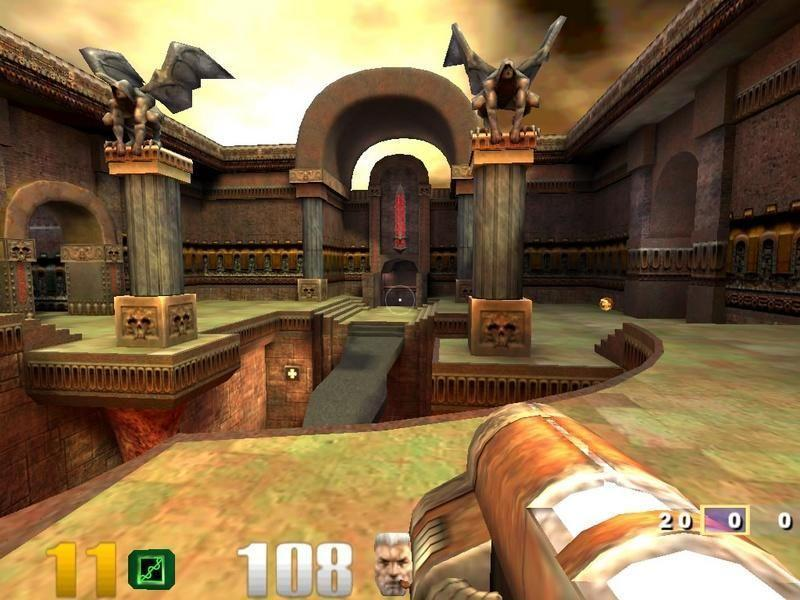
\includegraphics[width=8cm]{quake3}
		\caption{Quake III Arena, kép forrás: id Software\cite{pic-quake3}}
	\end{figure}
	
	\subsection{Fast Inverse Square Root algoritmus}
	Miért van erre szükség?
	
	Shaw : The Legendary Fast Inverse Square Root cikke így beszél az algoritmusról\cite{FISR}:	
	Az inverz négyzetgyök számítása egy nagyon fontos része a számítógépes játékok fejlesztésében.
	\begin{itemize}
		\item \emph{Pathfinding}\footnote{A mesterséges intelligencia útkeresése.}
		\item Grafikus számítások (Fény, visszaverődések stb.)
		\item Egyéb vektornormalizációs műveletek, melyekhez szükséges a számításban.
	\end{itemize}
	Grafikailag intenzív játékokban, pont mint a Quake III Arena, ezek a számítások másodpercenként akár milliószor is megtörténhetnek, így ezen a számításon optimizálást végrehajtva hatalmas teljesítményjavulást tudunk elérni.
	
	De hogyan is csinálták az \emph{id Tech 3} játékmotor programozói, hogy felgyorsították az időben drága inverz négyzetgyökszámítást?
	Implementáltak egy nagyon gyors és pontos közelítést erre.
	Lényegében egy \emph{Newton-Raphson iteráció} alapú közelítésről beszélünk.
	
	\begin{definicio}
		\label{def-NRI}
		Newton-Raphson gyökkeresés:
		Megkapjuk egy szám közelítését, és egy jobb közelítést érünk el:
		
		\begin{math}
			y = c/2 * (3 — xc^2) 
		\end{math}
	\end{definicio}

	A Fast Inverse Square root pedig az iterációt egy nagyon okos tippel kezdi.
	A kód megtekinthető itt[\pageref{kod-FISR}].
	
	Ez a kód jelentős, és legendás státuszt ért el a játékfejlesztés történelmében. ,,Fekete mágiának" tartott géniuszi bitmanipulációja és technológiai jelentősége miatt kapott hírnevet. A régebbi processzorok számára ez hatalmas teljesítmény növekedés volt, ám később, 1999-ben az \emph{Intel} által kiadott processzorok számára már elavulttá vált ez a művelet. Újabb műveletek már az idő tizede alatt sokkal kevesebb hibával is el tudták ezt érni. Pontosabb számítások esetére is találtak megoldást ami a \emph{FISR} algoritmus sebességének 80\%-ával el tudott érni \begin{math}<0,01\%\end{math}-os hibaszázalékú megoldást.
	
	\begin{lstlisting}[language=C, caption={Fast Inverse Square root algoritmus, cenzúrázva}, label=kod-FISR, float, floatplacement=hbt, captionpos=b]
		float Q_rsqrt( float number )
		{
			long i;
			float x2, y;
			const float threehalfs = 1.5F;
			
			x2 = number * 0.5F;
			y  = number;
			i  = * ( long * ) &y; // evil floating point bit level hacking
			i  = 0x5f3759df - ( i >> 1 ); // what the ****? 
			y  = * ( float * ) &i;
			y  = y * ( threehalfs - ( x2 * y * y ) ); // 1st iteration
			//  y  = y * ( threehalfs - ( x2 * y * y ) ); // 2nd iteration,
			// this can be removed
			
			return y;
		}
	\end{lstlisting}
	\pagebreak

	\subsection{Half-Life és a realizmus}
	A Half-Life sorozat mondhatni az egyik leglényegesebb, ha nem a leglényegesebb játéksorozat a '90-es évek végéről és a 2000-es évek elejéről.
	
	A realizmus pedig rég célja a játékoknak. Bár nem feltétlenül szükséges egy játéknak, hogy realisztikus legyen ahhoz, hogy élvezhető legyen, de lenyűgöző és bevonzó lehet egy játék minél hűebb a valósághoz.
	
	Matthew Byrd cikke\cite{HL} alapján:
	Az első rész a sorozatban, szimplán Half-Life, 1998-ban jelent meg. Az elterjedt közös megegyezés az, hogy nagyon fejledt játék volt az idejéhez képest és sok innovációt hozott be, bár arról már kevesebbet beszélnek manapság.
	
	A \emph{Half-Life} volt az a játék a '90-es években, ami lefektette az alapjait annak, hogy, hogyan definiálunk, mi tesz egy PC játékot PC játékká, emellett még egy olyan tapasztalatot nyújtott a játékosok számára, amit abban a korban nem sok fejlesztőcsapat tudott volna nyújtani.
	
	\begin{figure}[!ht]
		\label{kep:hl1}
		\centering
		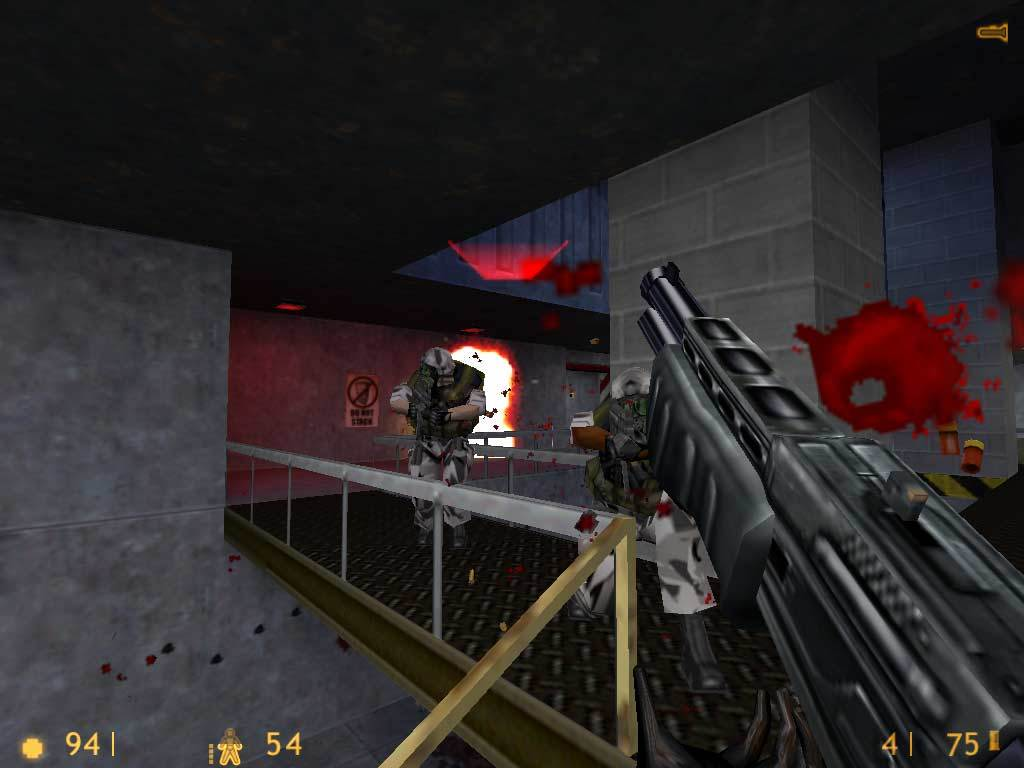
\includegraphics[width=8cm]{halflife1}
		\caption{Half-Life (1998), kép forrás: Valve\cite{pic-HL}}
	\end{figure}
	
	Gránátok dobásától \emph{játék modolhatóságig}\footnote{A modolhatóság annyit jelent, hogy felhasználói módosításokat adhatunk hozzá, akár sajátot vagy másét.} nagyon sok olyan fogalmat hozott be, amelyeket a mai napig használnak a modern játékokban.
	
	Mai viszonylatban elég viccesnek tűnik, de a játék használati utasításában az van kiemelve realisztikus ténynek, hogy a játékban található fegyverek logikusan vannak elhelyezve és nem csak lebegnek, mint például a Quake játékokban általánosan.
	
	Az emberi ellenséges entitások mesterséges intelligenciája már képes volt reagálni a gránátok jelenlétére és a saját életüket helyezték előre, míg az űrlények pedig nem futottak el a gránátok elől mert ugye nem tudják mi az.
	
	\subsection{Half-Life és a map design}
	
	Előtte kiadott játékok, mint például az \emph{Unreal}, \emph{Doom}, \emph{Hexen} igazából nem szenvedett rossz pályafelépítésekkel, vagyis \emph{map design}-al, de nem igazán adták át a pályáik, hogy egy nagyobb világ részét képeznék.
	
	A Half-Life ezt teljesítette pár szóra érdemes módon:
	\begin{itemize}
		\item A technikai oldalon: A Valve egy eléggé nagy világot teremtett, és ennek a töltése a háttérben történik.
		Ez azt jelentette, hogy a felhasználóknak jóval kevesebbet kellett töltőképernyők előtt ülniük. Így sokkal jobban bele tudta élni magát a játékos, hogy egy kutatási központot kell navigálnia, és nem egy tradicionális szintről szintre lépkedéses megoldásban történt, mint például a \emph{Doom}-ban.
		
		\begin{figure}[!ht]
			\label{kep:hl2}
			\centering
			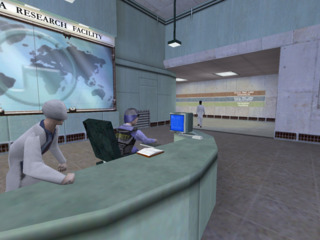
\includegraphics[width=8cm]{halflife2}
			\caption{Half-Life (1998) Black Mesa kutatóközpont, kép forrás: Valve, giantbomb.com\cite{pic-hl2}}
		\end{figure}
		
		\item A teljes innováció azonban túllő csak a technikai oldalon. A Half-Life csapata, úgy készítette el a pályákat, hogy úgy tűnjön, hogy a kutatási központ minden részének külön feladata, jelentősége van. Ez egy nagyon fontos pályadizjánolási pont, hogy hihető legyen, hogy az a pálya miért van ott, és hogy úgy érződjön, hogy igen, ennek ott kell lennie. Direkt úgy építették össze a pályákat, hogy hihető legyen, hogy az egy kutatási központ:
		\begin{itemize}
			\item Laborok egymés mellett, amik hasonló anyagokat tanulmányoznak.
			\item Pihenőszobák.
			\item Raktárok, raktárterületek.
		\end{itemize}
	\pagebreak
	\end{itemize}
	
	\subsection{Half-Life modolhatósága}
	Fontos, hogy emellett a Half-Life másik nagy innovációja, a \emph{modolhatóság}.
	\begin{definicio}
		Modolás:
		Modolás alatt modifikációra utalunk, ami a játékok értelmében pályák hozzáadását, teljesen új \emph{kampányt}\footnote{Kampány alatt a játék fő sztorivonalát értjük.}, új fegyvereket és ilyesmi új lelkes felhasználók által hozzáadott tartalmat értünk.
	\end{definicio}

	A Valve meghozta azt a döntést, hogy a közösség kezébe ad egy könnyebb hozzáférést a játéktartalom gyártásához a dizájnprogramokkal, amiket használtak a játék elkészítéséhez.
	Ilyen például a \emph{Hammer}. A \emph{Hammer} egy pályaszerkesztő-készító program, mellyel GoldSource pályákat tudunk készíteni.
	
	Később a Valve is, de több játékstúdió is rájött, hogy nem csak arra vannak a vásárlók, hogy megvegyék a játékot, hanem modolhatóság által még a játékban bent maradt hibákat is megoldhatják, amennyiben zavarja őket, nem csak textúrákat fognak kicserélni, hanem akár teljesen új tartalmat és tapasztalatokat is generálhatnak a játék alapján.
	
	\section{Játékmodifikációk jelentősége}
	
	A játékmodifikációk nagyon lényegesek a fejlesztők számára, mivel, ha valakit inspirál egy játék arra, hogy változtasson benne valamit, akkor rávezeti arra, hogy tanuljon játékfejlesztést valamilyen szinten.
	
	Mellékhatásként, még a játék körüli közösséget is fenntartja, és élettelibbé tehetik akár évekig az ilyen modok, mivel így a játékosok a saját tetszésüknek megfelelővé tehetik vele a játékokat.
	
	Általában sokkal könnyebb a fejlesztés, ha az ember olyan dologgal foglalkozik, amit szeret úgynevezett \emph{modderek}, akiket fel is vettek az adott céghez dolgozni, például az eredeti \emph{TF Software}-ből \emph{Robin Walker és John Cook}, akik elkészítették eredetileg a Team Fortress mod-ot, még a \emph{Quake}-hez, később a Team Fortress: Classic-ot GoldSource-ra, mégkésőbb a Team Fortress 2-t a Source motorra, az utóbbi kettőt már a Valve szárnyai alatt tették.
	
	Az előbb említettet belevonva, sok olyan modder vagy modoló csapat van, akik átmentek arra, hogy felépítsék a saját különálló játékukat a modjuk alapján.
	
	Ilyen például a \emph{The Forgotten City} mod\cite{mod-forgcity}, ami már szimpla mod státuszában is sok díjra lett jelölve a közösség által, melynek készítője később egy stúdióval megalkotta a saját önálló játékát ugyanezen a néven.
	
	
	\begin{figure}[!ht]
		\label{kep:forgcity1}
		\centering
		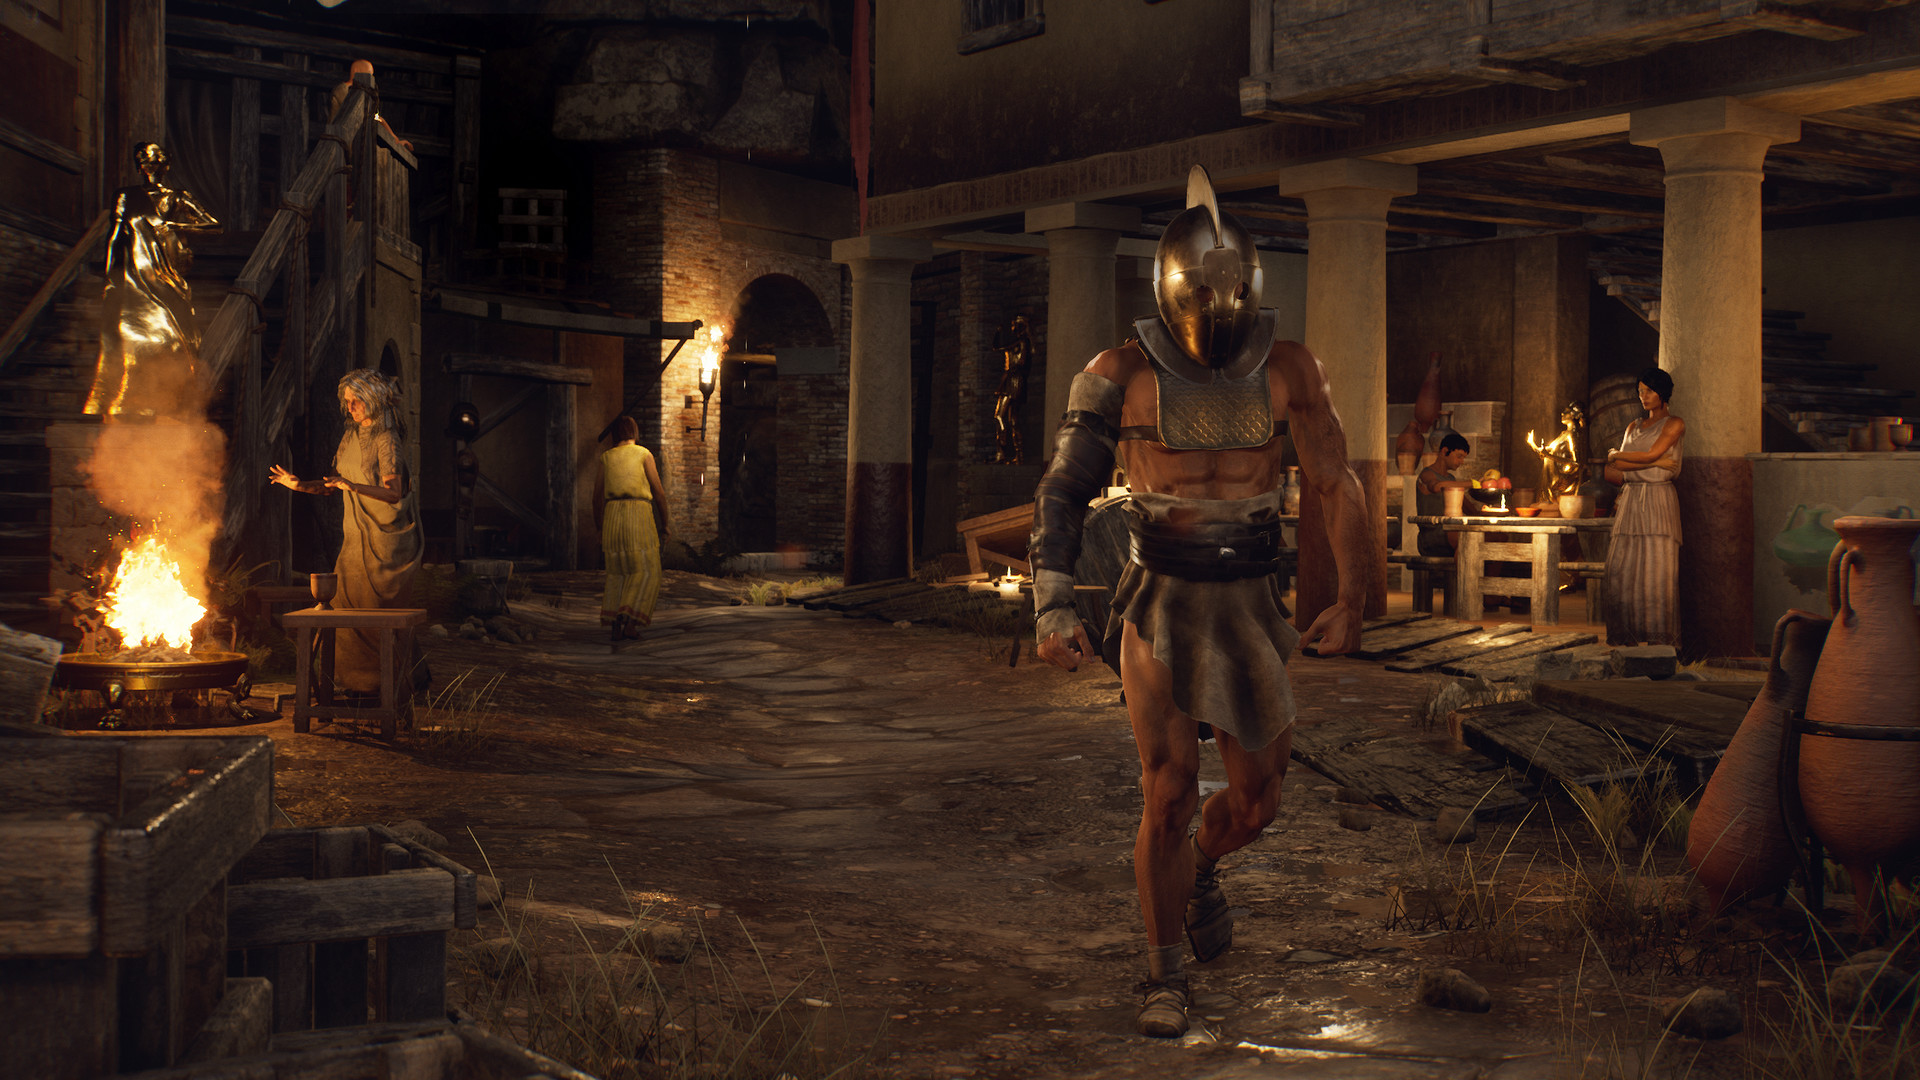
\includegraphics[width=8cm]{forgcity1}
		\caption{The Forgotten City (2021), kép forrás: Modern Storyteller\cite{pic-forgcity}}
	\end{figure}
	
	Ezekbe a sikerekbe belegondolva, a játékmodifikációk gyártása nem tűnik annyira vesztegetett időnek, mivel sok játékfejlesztő cég erre, úgy figyel mint egy tehetségkutató, mint például a \emph{Bethesda Softworks} a mérhetetlen mennyiségű modifikációkkal a játéksorozataikra, akik \emph{Todd Howard} szavaival élve, már több alkalommal vettek fel új dolgozókat a játékaikat modifikáló felhasználók közül, amennyiben nyilván megfeleltek a munkakör feltételeinek. Ezáltal mondható, hogy a játékmodifikációk gyártása lehet egy egyenes út a professzionális játékfejlesztésbe is.
		
	\section{Játékmotorok}
	\begin{definicio}
		Játékmotor:
		A játékmotor lényegében egy keretrendszer a játékok fejlesztésére.
	\end{definicio}
	
	A játékmotorok ma már szerves részét képezik a játékfejlesztésnek, azonban régebben nem voltak külön játékmotorok fejlesztve.
	A játékmotorok mint, szó a '90-es években kezdett el terjedni, ennek a fő oka a \emph{DOOM} játék fejlesztése és a \emph{DOOM Engine}.
	
	\subsection{Játékmotorok feladata}
	A játékmotorok általános feladata az, hogy megkönnyítsék a játékfejlesztést a fejlesztők számára. Vannak komplett játékmotorok, amik a játékfejlesztés legnagyobb pontjait lefedik, de vannak specializálódottabb motorok, mint például grafikai motorok, ilyen az \emph{Unreal}.
	
	Általában úgy fejlesztik ki ezeket a motorokat, hogy alapból rendelkezzenek olyan modulokkal, amik nagyon hasznosak a játékfejlesztésnél. Például manapság már általában, ilyen modulok vannak beépítve:
	
	\begin{itemize}
		\item Fizikai rendszer (Gravitáció, ütközés stb.)
		\item Árnyékolási rendszer
		\item 2D, 3D grafikai rendszer
		\item Hangrendszer
	\end{itemize}
	Gyakran ezek funkcionalitása részben felül is írható, ezzel is egyedivé tehetőek a játékprojektek.
	
	\subsection{DOOM Engine}
	\emph{Henry Lowood} cikke szerint:\cite{doomengine}
	A játék 1993-as kiadási dátuma előtt id Software kiadott egy olyan kijelentést, hogy a technológiájuk ki fogja terjeszteni az általunk képzelt limitáltságát a számítógépes játékoknak.
	
	Ez a nyilatkozat hozott be egy új fogalmat, a ,,DOOM Engine" és az ,,engine" fogalmát.
	Ez az új fejlemény megformázta a játékfejlesztés jövőjét és újratervezte a játékfejlesztés iparát.
	
	A játékmotor fogalom létrehozása mellett, \emph{John Carmack}, vezető programfejlesztő az id Softwarenél, nem csak egy új szoftvert hozott létre, hanem ezzel a motorral, jól definiáltan, szét is választotta a belső működéseket, mint például a 3D megjelenítő rendszert, játéklogikát a kreatív tartalmaktól mint például a textúráktól.
	
	A DOOM-motor C és Assembly nyelven íródott.
	
	\subsection{Unreal Engine}
	Az Unreal Engine (UE) egy 3D számítógépes grafikai játékmotor, melyet az \emph{Epic Games} fejlesztett ki. Először a saját 1998-ban kiadott \emph{Unreal} belsőnézetes lövöldözős játékukban mutattak be. Készítője: \emph{Tim Sweeney} és C++-ban íródott.
	
	\begin{figure}[!ht]
		\label{kep:unreal1}
		\centering
		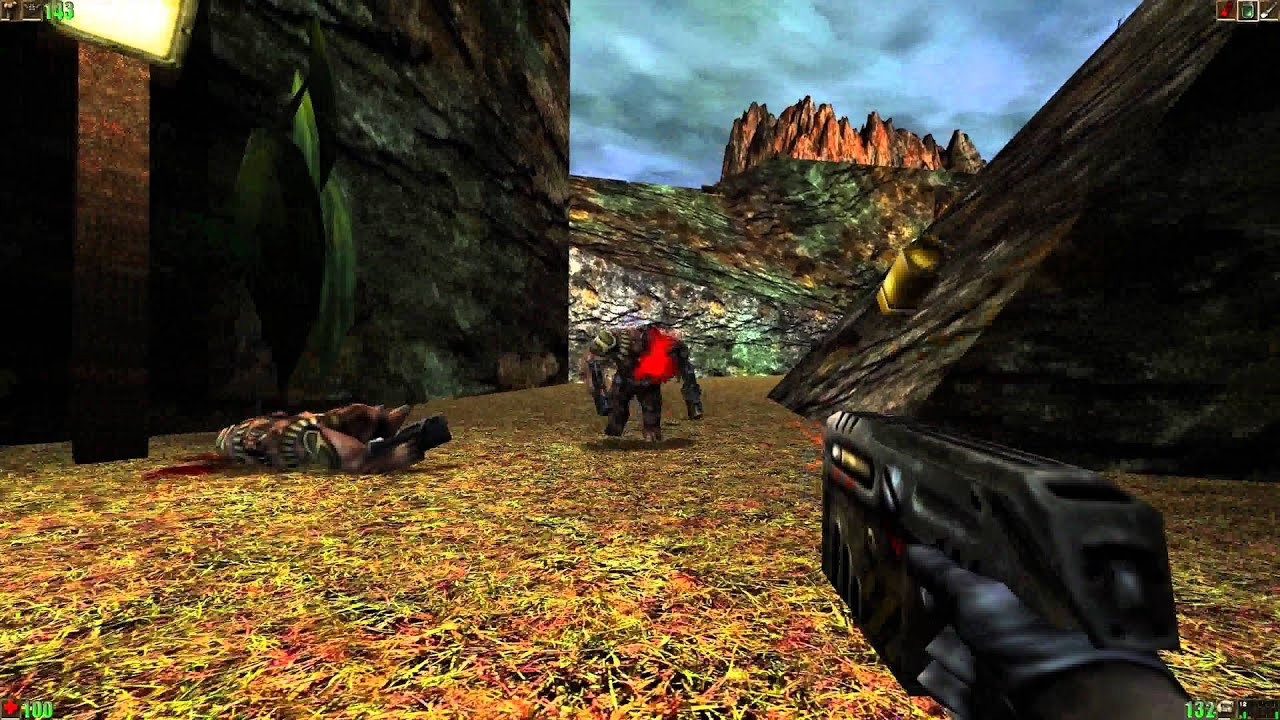
\includegraphics[width=8cm]{unreal1}
		\caption{Unreal (1998), kép forrás: Youtube: Methos és Epic Games\cite{pic-unreal1}}
	\end{figure}
	
	Az Unreal Engine gyorsan kinőtte magát abból, hogy egy játékstúdió motorja, és ma már megszámlálhatatlan mennyiségű játék használja grafikai alapjaként a motort. Például:
	
	\begin{itemize}
		\item Mass Effect széria
		\item Life is Strange
		\item Dishonored
	\end{itemize}
	
	2023-ban már az 5.0-ás verzióról beszélünk az Unreal Engine 5-ről, mely képességéről már nehézség megmondani, hogy a valóságról beszélünk-e, vagy egy gép által renderelt virtuális valóságról.
	
	\begin{figure}[!ht]
		\label{kep:unreal2}
		\centering
		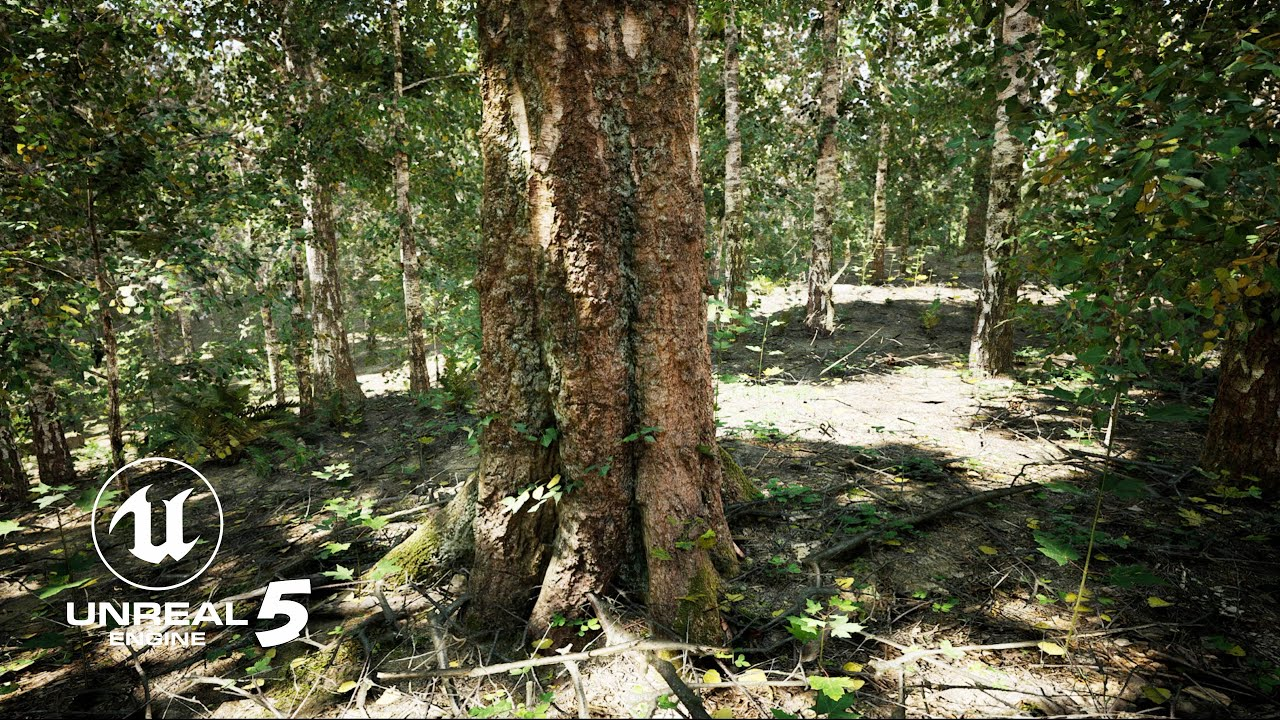
\includegraphics[width=8cm]{unreal2}
		\caption{Unreal Engine 5, kép forrás: Youtube: JSFILMZ és Epic Games\cite{pic-unreal2}}
	\end{figure}

	\subsection{Unity Engine}
	A Unity egy \emph{cross-platform}\footnote{A cross platform annyit jelent, hogy több platformon is futtatható/elérhető az alkalmazás.} játékmotor, amit 2005-ben adott ki a Unity Technologies, lényegében arra, hogy ,,demokratizálja" a játékfejlesztést.
	
	A Unity Engine egy teljesjogú játékmotor, több modulja is van, ami segíti a játékfejlesztést:
	
	\begin{itemize}
		\item Fizikai rendszer (Gravitáció, Collision, stb.)
		\item Hang, hang-event rendszer.
		\item Animációk, animáció recording.
		\item Felhasználói felület gyártás.
		\item Pályadizájn segítés
		\item Mesterséges intelligencia segítség (Navmesh generálás, stb.)
	\end{itemize}
	
	Hatalmas hírnévre tett szert ez a játékmotor, mivel elérhetőbbé tette a játékfejlesztést mindenki számára, még annak is, akinek elérhetetlen lett volna alapból és még meg is könnyítette. Már készen álló, de felülírható beépített moduljai sokban segítik a játékfejlesztés folyamatát.
	
	2005-ben adták ki az 1.0-ás verziót, eredetileg egy Mac OS X játékmotorként. Jelölve is lett az Apple Design Awards díjazásra a legjobb grafikai használatért. Később kapott támogatást Windows-ra, Linuxra és böngészőkre is.
	
	A Unity alapjáraton használható két dimenziós és három dimenziós játékok fejlesztésére is, mivel mindkettőre ad akkomodáló modulokat.
	
	A Unity 2.0 2007-ben jött ki és már erősebb támogatást adott a háromdimenziós játékok fejlesztésére, optimizált terraformálás, valós idejű dinamikus árnyékok és még sok más. Ez a verzió azért is fontos, mivel 2008-ban adta ki az Apple az Apple Store-t és a Unity pedig rohamtempóban támogatást adott ki rá. Ezzel elterjedt az \emph{iOS} fejlesztők körében is.
	
	Egy 2012-es kutatás szerint\cite{unitysurvey} a mobiljátékfejlesztés nagyon az iOS és Unity összeállítás irányába haladt. A fejlesztők, akiket megkérdeztek 94,6\%/ban iOS-re fejlesztettek, ezzel az lett a legelterjedtebb platform, az android pedig második helyen 70,7\%-ban. A játékmotorokat tekintve pedig a Unity lett a legelterjedtebb 53,1\%-os fejlesztői aránnyal, második helyen pedig saját motort használtak 39,8\%-al.
	
	Fejlődése során, mivel alapelve az inkluzivitás a platformok felé, kibővítette a támogatott platformok listáját. Mára már mobil és pc támogatás mellett támogat webes, konzol és virtuális valóság platformokat is.
	
	\begin{itemize}
		\item Mobil
		\begin{itemize}
			\item iOS
			\item Android
			\item tvOS
		\end{itemize}
		\item Asztali
		\begin{itemize}
			\item Microsoft Windows
			\item Mac
			\item Linux
		\end{itemize}
		\item Web paltform : WebGL
		\item Konzol platformok
		\begin{itemize}
			\item Playstation
			\item Xbox
			\item Nintendo Switch
			\item Stadia
		\end{itemize}
		\pagebreak
		\item VR,ER
		\begin{itemize}
			\item Oculus
			\item Playstation VR
			\item ARCore
			\item ARKit
			\item Windows Mixed Reality
			\item Magic Leap
			\item SteamVR
			\item Google Cardboard
		\end{itemize}
	\end{itemize}
	
	\chapter{Unity Játékfejlesztés menete és kivitelezése}
	A téma kiválasztásánál fontosnak tartottuk, hogy a kettőnk feladata könnyen összeilleszthető legyen és, egy olyan játékmotort válasszunk, ami kellően támogatja mindkettőnk tevékenységét. Ezért választottuk a Unity-t.
	
	Kiskorom óta szerettem a két dimenziós platformer játékokat, így biztosra tudtam, hogy azt szeretnék csinálni erre a projektre.
	
	\section{Tervezés}
	Először inspirációt gyűjtöttem más hasonló játékokból. Ilyen például a \emph{Super Mario}, ami a számítógépes játékokba az egyik bevezető játékom volt, a második pedig a \emph{Shovel Knight} 
	
	\begin{figure}[!ht]
		\label{kep:shovelknight}
		\centering
		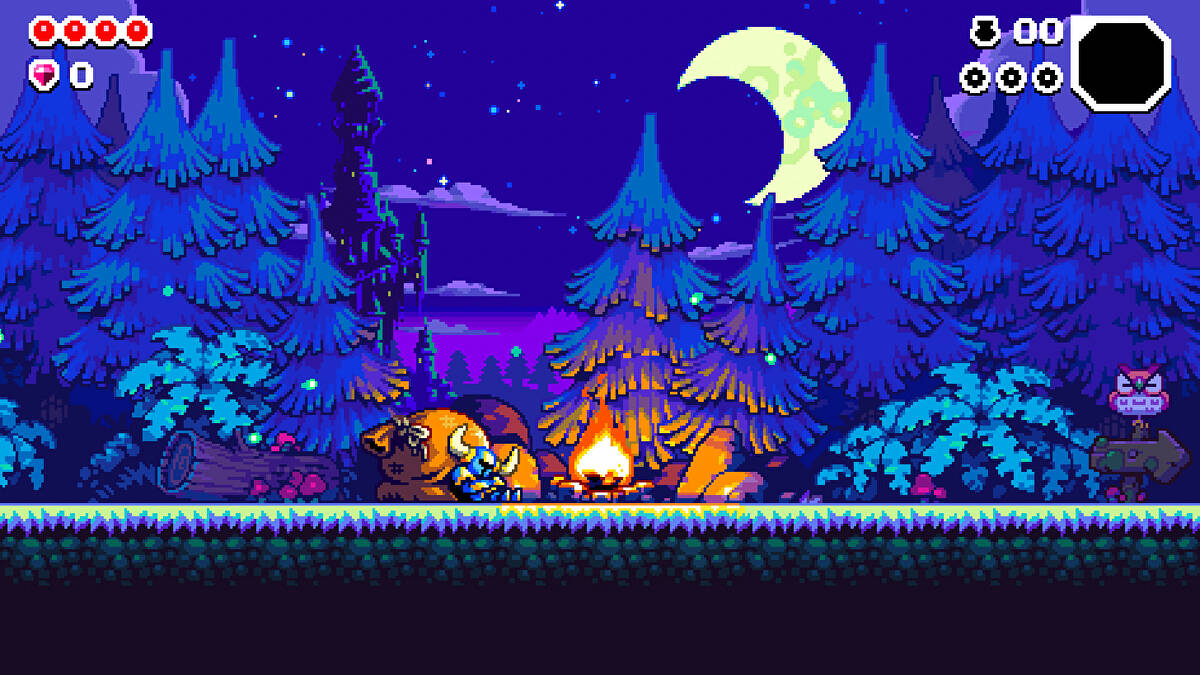
\includegraphics[width=8cm]{shovelknight}
		\caption{Shovel Knight (2014), Yacht Club games forrás: https://www.eurogamer.net/shovel-knight-dig-a-great-series-safe-in-the-hands-of-the-very-bests}
	\end{figure}

	A \emph{Shovel Knight} a modernebb két dimenziós platformer\footnote{A Platformer játékok, olyan játékok, melyek pályak pálya alapú manőverezési problémákat tesznek fel.}, amely egész nagy sikereket ért el a piacon.
	
	Lényegében ez a két játék inspirált engem arra, hogy én is egy két dimenziós platformer játékot készítsek.
	
	Az előző nyár alatt sokat kutattam a Unity játékfejlesztéssel kapcsolatban. Elveket a pályatervezéssel kapcsolatban, hogy milyen nehézségűnek kell a pálya bejárásának lenni, hogy élvezhető legyen.
	Hogyan kell a játékost mozgatni és a többi.
	
	
	Először, a tervezéseink szerinti menüt terveztük ki.
	
	\begin{figure}[!ht]
		\label{kep:mainmenuusecase}
		\centering
		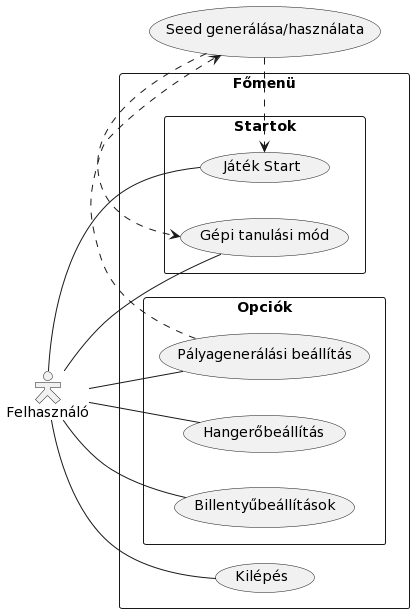
\includegraphics[width=8cm]{MainMenu_usecase}
		\caption{Főmenü Use-case}
	\end{figure}

	Úgy terveztük, hogy eredetileg randomizált legyen a pályagenerálás, de ezt az ötletet eldobtuk. A játékot két módban lehet elindítani:
	
	\begin{itemize}
		\item Alapjáték -- Játékos irányítja a karaktert.
		\item Gépi tanulási mód -- Gépi tanulás algoritmus kezeli a karaktert.
	\end{itemize}

	Hangbeállításoknál a zene és zajok hangosságának átállítására van esélyünk. Billentyűbeállításoknál pedig a támadás és ugrás gombját tudjuk átállítani. A kilépés pedig szimplán bezárja az alkalmazást.
	
	A főmenü megtervezése után pedig a játékos mozgatását kezdtem el kutatni, hogy, hogyan kellene megoldani.
	
	Először megterveztem egy UML-t arról, hogy mit is szeretnék elérni.
	Alapjáraton, mivel egy két dimenziós játékról beszélünk, így balra, jobbra mozgást kell nyújtanunk, valamint ugrásra lehetőséget.
	
	\begin{figure}[!ht]
		\label{kep:movementusecase}
		\centering
		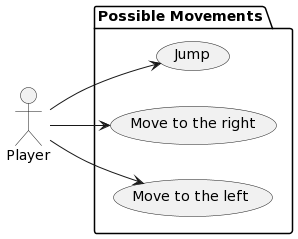
\includegraphics[width=8cm]{movementusecase}
		\caption{Use-case ábra a mozgásról való elképzelésről.}
	\end{figure}

	Ezek mellett természetesen le kell majd kezelnünk, olyan helyzeteket, mikor a játékos modelljét meg kell fordítanunk, hogy a haladás irányába legyen fordulva.
	
	Ennek a segítségére felhasználtam \emph{Pandemonium} Unity játékfejlesztési tutorialját használtam fel.\cite{vid-unity1} ettől a videótól teljesen megértettem, hogy, hogyan kellene megvalósítanom az eltervezett mozgást a játékos számára és le is kezelte a model megfordítási problémám.
	
	A mozgások mellett szükség lenne persze az animációkra is a mozgásokhoz, szerencsére alapvető tudást megadta ez a videó is, és ebből képes voltam tovább építkezni az ötleten.
	
	Lényeges alapja lenne a játékomnak a támadás is, és erre is keresnem kellett egy jó megoldást. Én \emph{Brackeys} videóját találtam a legtalálóbbnak és számomra szimpatikus megoldásnak.\cite{vid-unity2}
	A videó informatívan és követhetően magyarázza el a mögötte álló technológiát, és, hogy azt, hogyan kell használni általánosságban.
	Kellően jó megoldást adott a tipikus hibákra mint több ellenfél eltalálásának a működése, és hogy alapjáraton mivel detektáljuk, hogy eltaláltuk-e az ellenséget. Ezáltal el is tudtam készíteni egy aktivitás diagramot, hogy, hogyan szeretném, hogy működjön a játékos támadása.
	
	\begin{figure}[!ht]
		\label{kep:attackchart}
		\centering
		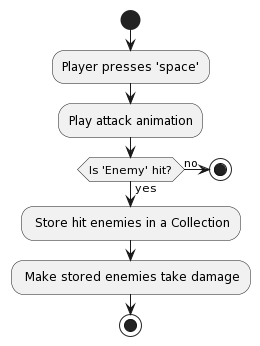
\includegraphics[width=8cm]{attackchart}
		\caption{Aktivitás diagram a játékos támadásáról.}
	\end{figure}
	
	\pagebreak
	Felvehető tárgyakat is terveztem, mivel ezzel érdekesebbé is tudjuk tenni a játékot a játékos számára.
	
	Tesztelésképp az elején, csak egy olyan tárgyat tervezek, ami csak visszadob a pálya elejére. Később viszont, már olyanokat is tervezek, amiktől a játékos többet fog sebezni, több életereje lesz és esetleg egy értéket képező felvehető tárgy, ami növeli a játékos pontszámát. A játékos pontszáma pedig, csak annyi funkciót lát el, hogy visszajelzés a játékosnak, hogy mennyire fedezte fel a pályákat.
	
	Fontos része a tervezésnek még, hogy össze kellett gyűjteni olyan ,,asset"-eket, amelyeket használni fogok a játék fejlesztésekor.
	Mikor ezeket összegyűjtöttem, figyeltem arra, hogy kizárólag ingyenesen használható tartalmakat használjak fel.
	
	Erre a \emph{Unity Asset Store}-t használtam fel. Ez a Unity saját \emph{asset} megosztó platformja, ahol a készítők akár értékesíthetik az általuk gyártott tartalmakat, melyek felhasználhatók a játékok fejlesztéséhez.
	\pagebreak
	
	A keresett asset-ek főleg:
	
	\begin{itemize}
		\item Protagonista modell
		\item Ellenség modell
		\item Textúrák
		\begin{itemize}
			\item \emph{Skybox}\footnote{Az eget szemléltető kép.}
			\item Talaj, falak
			\item Opcionális szépítések.
		\end{itemize}
		\item Felhasználói felület
	\end{itemize}
	
	\section{Verziókövetés}
	A Unity projektek számára az ajánlott a \emph{Unity Version Control}, régebbi nevén \emph{Plastic SCM}. Mi azonban, egy különlegesen erre összerakott \emph{gitignore} fájllal ellátott \emph{Git}-et használtunk, projektünket \emph{GitHub}-ra tettük fel, ahol publikusan elérhető \emph{repository}-ban elérhető:
	\url{https://github.com/O48WRX/Szakdoga}
	
	Azért választottuk a Git és GitHub kombinációt, mivel ez számunkra a megszokott, és mindenféleképpen a zökkenőmentes, stabil együttműködést szerettük volna elérni.
	
	A Git nagy előnye, hogy könnyen kezelhető terminálból, de nagyon sok \emph{IDE} \footnote{Integrated Developer Environment, integrált fejlesztési környezet.} alapjáraton támogatja a Git-et.
	
	Tudja segíteni a csapatmunkát azzal is, hogy beépített feladatkövető rendszere is van, mellyel folytonossá és könnyűvé teszi a csoportos munkákat.
	
	\section{Csapatmunka}
	Programfejlesztők folyamatosan csoportos munkával fognak találkozni a munkahelyen, így nagyon örültem a lehetőségnek, hogy a konzulensem mellett csapatként is dolgozhatok hallgatótársammal ezen a témán.
	
	Egyetemen is már többször kellett csoportos munkában részt vennünk, de ebben az esetben ez a téma túlfed egy félévet a súlyával, így teljesen kiteljesedve tudunk dolgozni a témán, érezve a végeredmény komolyságát is.
	
	Nagyon fontos csapatmunkánál a kommunikáció, így törekedtünk arra, hogy legalább hetente kétszer konzultáljunk egymással a helyzet állásáról.
	
	Első elképzelésekkel ellentétben nehezebbnek bizonyult a csapatmunka, mivel még nem dolgoztunk ekkora projekten, így sok személyes faktorhoz hozzá kellett szoknunk.
	
	\pagebreak
	
	\section{Csapatbeli kommunikáció}
	Mivel csoportos munkánál a kommunikáció kifejezetten fontos szerepet kap, így mi is nagy fókuszt raktunk erre a részére a csapatmunkának.
	
	Gyakran téma volt nálunk személyesen is, amikor találkoztunk egyetemen vagy egyéb eseményeknél is, hogy, hogyan kellene továbbfejleszteni a projektünket. A tervezés nagy része viszont, főleg a \emph{Discord} alkalmazáson történt, vagy a \emph{Meta Messenger} alkalmazásán történt.
	
	Messengeren a kisebb változásokat beszéltük meg, vagy kisebb betervezett \emph{feature}-öket. A főbb tervezések Discord-on történtek, ott beszéltük meg az eredeti műfaját a játéknak és, hogy milyen funkciókat fog tartalmazni például.
	
	\section{Feladatok megosztása}
	A tervezésünk egyik legfontosabb része volt, mivel arra kellett odafigyelnünk, hogy fair módon osszuk el egymás között a feladatokat. Mivel ketten voltunk egészen könnyen el tudtuk felezni a felelősségeket egymás között.
	
	Mivel egészen hamar eldöntöttük, hogy ki melyik részét fogja csinálni a projektnek, én magát a játékot, Henrik pedig a mesterséges intelligenciát és a gépi tanuló algoritmust, így ezzel a részével nem kellett küzdenünk.
	
	Viszont a nehézségek a feladatok heti leosztásánál voltak, mivel ebbe külső hatások is belekavartak, mint a családi és egyéb programok és maga az egyetem is. Ezért gondoltam szükségesnek, hogy megemlítem ezt a részét is a fejlesztésnek.
	
	\section{Fejlesztés}
	
	\subsection{Főmenü}
	A legelső amit elkészítettem aza főmenü volt. Elemi része a játékoknak a főmenü, hogy el lehessen indítani a játékot, tetszőleges beállításokat végezni a játék működésén vagy működtetésén.
	
	\begin{figure}[!ht]
		\label{kep:mainmenu}
		\centering
		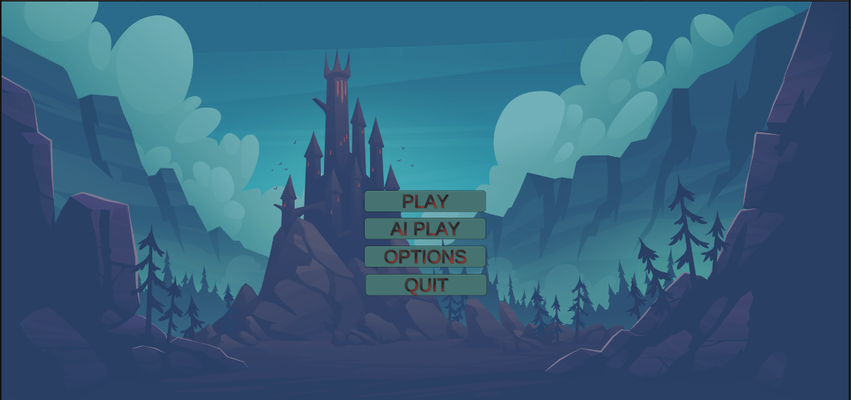
\includegraphics[width=8cm]{mainmenu}
		\caption{A játék főmenüje.}
	\end{figure}
	\pagebreak
	Fő feladat az volt a menünél, hogy ez legyen az első \emph{scene}\footnote{A scenek, az, az jelenetek, a Unity-ben az elkészített pályák technikailag, amik között váltogatni tudunk.} és itt lehessen beállítani a hangerőt, valamint, hogy az indítógombbal az első pályára kerüljünk át. Ezt egy szimpla sor kóddal el lehet érni:
	
	\begin{lstlisting}[breaklines=true, caption={A játék Scene léptető kódsora.}, captionpos=b]
public void playGame()
{	
	SceneManager.LoadScene(SceneManager.GetActiveScene().buildIndex + 1);
}
	\end{lstlisting}

	\subsection{Platformok}
	A főmenü után, első feladatom az volt, hogy előállítsak egy navigálható tesztpályát. Először \emph{platformokat}\footnote{A navigálható felületeket, amivel ütközik a játékos.} kellett létrehoznom. Erre felhasználtam a Unity-be beépített \emph{Square} objectet, melyet transzformálva elértem a szükséges kinézetet. Ezeknek a platformoknak a pozíciója abszolút és nem megváltoztatható a játékos által. A transzformálására, a beépített \emph{Transform} komponenst használtam fel, láthatóságára/színezésére pedig a \emph{Sprite Renderer} komponenst. Itt még fennállt az a probléma, hogy a játékos átesett az objektumon, ezért még a \emph{Box Collider 2D}-t is felhasználtam, ezzel kiküszöböltem a játékos és egyéb \emph{Actor}-ök átesését.
	
	A \emph{Box Collider 2D} az egyik legfontosabb eszköz, amit használtam a játék fejlesztése során. Megoldja, hogy a karakterek ne tudjanak átesni a \emph{Collision Box}-án, ami skálázható méretű, valamint a \emph{Material} property-jével megoldható az \emph{Actor}-ök falon való fennakadása. Ez úgy történik, hogy mind a platformok és a játékos és az NPC-k\footnote{Non-Player Character, nem a játékos által irányított karakterek.} is el vannak látva \emph{Collision Box}okkal, skálázva a modellekhez, és a kettő doboz nem tud átesni egymáson.
	
	
	\begin{figure}[!ht]
		\label{kep:platform}
		\centering
		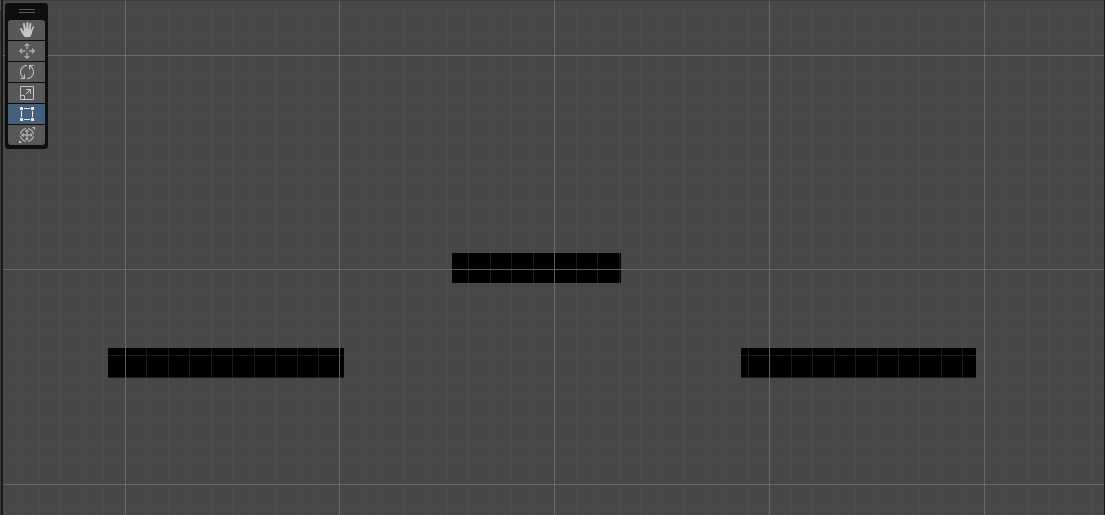
\includegraphics[width=8cm]{platforms}
		\caption{Az első tesztpályán (TestMap01) lévő platformok}
	\end{figure}

	\section{Játékos}
	A játék egyik legfontosabb része, minden bizonnyal, hogy legyen egy játékos által irányítható objektum, amivel játszhatja a játékot. Alapjáraton, egy a platformokhoz hasonlító fekete négyzet volt a játszható karakter.
	\subsection{Mozgás}
	A játékos mozgása elemi része az ilyen játékoknak, mivel az élvezhetőségének az egyik alapja.
	Legelőször a gravitációt kellett implementálni.
	\subsubsection{Gravitáció}
	A gravitációt, úgy oldottam meg, hogy a játékos objektumnak adtam, egy \emph{Box Collider 2D}-t, hogy ne essen át a platformokon, ezután felhasználtam a \emph{Rigidbody 2D} komponenst, melyben a ,,Body Type"-ot dinamikusra állítjuk és ez alapjáraton rendelkezik egy ,,Gravity Scale" property, mely alapjáraton ellátja az objektumunkat egy Y tengelyen való mozgással.
	
	\subsubsection{Kétirányú mozgás}
	A kétirányú mozgás, a futás szintén egy alapja, amihez már az X-tengelyen való mozgatás szükséges.
	
	Emellett még a modelltranszformáció is egy probléma amit meg kellett oldani. Ez annyit jelent, hogy az adott irányba való mozgásnál, az \emph{Actor}-ök modeljét az adott irányba kell elforgatni.
	
	\subsubsection{Ugrás}
	Az ugrás szintén, mivel platformer játékról beszélünk, alapköve a műfajnak, hogy a nehezebben elérhető, esetlegesen elrejtett részekre is el tudjon érni a játékos.
	
	Ezt a mozdulatot már az Y-tengelyen kell végezni, és egy folyamatosan csökkenő sebesség alapján kell számítani. Amikor az adott sebesség pedig eléri a 0-át, akkor pedig a beépített gravitáció vissza fogja húzni az objektumot.
	
	\chapter{Tesztelés}
	
	\begin{thebibliography}{2}
		\addcontentsline{toc}{chapter}{\bibname}
		\bibitem{textb-ag}
		\textsc{Sahith Dambekodi, Spencer Frazier, Prithviraj Ammanabrolu, Mark O. Riedl, Cornell University, arXiv:2012.02757}: \emph{Playing Text-Based Games with Common Sense}, 2020.12.04
		
		\bibitem{kutatas1}
		\textsc{infostart.hu, PopCap}:\emph{https://infostart.hu/eletmod/2011/11/27/kik-jatszanak-a-szamitogepes-kozossegi-jatekokkal-468037}
		
		\bibitem{vidgames}
		\textsc{Siyuan Xu}:\emph{ History of AI design in video games and its development in RTS games \text{https://sites.google.com/site/myangelcafe/articles/history\_ai}}
		
		\bibitem{FISR}
		\textsc{Shaw}:\emph{The Legendary Fast Inverse Square Root, https://medium.com/hard-mode/the-legendary-fast-inverse-square-root-e51fee3b49d9}, 2017.09.17
		
		\bibitem{HL}
		\textsc{Matthew Byrd}:\emph{Half-Life: The Forgotten Innovations of the PC Shooter, https://www.denofgeek.com/games/half-life-innovations-history/}, 2020.02.12
		
		\bibitem{doomengine}
		\textsc{Henry Lowood, Kinephanos, Stanford Libraries, Palo Alto}:\emph{Game Engines and Game History, https://www.kinephanos.ca/2014/game-engines-and-game-history/}
		
		\bibitem{unitysurvey}
		\textsc{gamedeveloper.com, Gamasutra}:\emph{Mobile game developer survey leans heavily toward iOS, Unity, https://www.gamedeveloper.com/audio/mobile-game-developer-survey-leans-heavily-toward-ios-unity}, 2012.05.24
		
		\bibitem{pic-HL}
		\textsc{Valve}:\emph{Half-Life (1998) kép, https://store.steampowered.com/app/70/HalfLife/?l=hungarian}
		
		\bibitem{pic-HL2}
		\textsc{Valve}:\emph{Half-Life (1998) kép, https://www.giantbomb.com/black-mesa-research-facility/3035-64/}
		
		\bibitem{pic-quake3}
		\textsc{id Software}:\emph{Quake III Arena (1999) kép, https://store.steampowered.com/app/2200/Quake\_III\_Arena/?l=hungarian}
		
		\bibitem{pic-unreal1}
		\textsc{Epic Games, Methos}:\emph{Unreal (1998) kép, https://www.youtube.com/watch?v=WTRmZ6aFEWM}
		
		\bibitem{pic-unreal2}
		\textsc{Epic Games, JSFILMZ}:\emph{Unreal Engine 5 kép, https://www.youtube.com/watch?v=1uXzaY749Ag}
		
		\bibitem{mod-forgcity}
		\textsc{TheModernStoryteller}:\emph{The Forgotten City, https://www.nexusmods.com/skyrimspecialedition/mods/1179}, 2016.10.29
		
		\bibitem{pic-forgcity}
		\textsc{Modern Storyteller, Dear Villagers}:\emph{The Forgotten City kép (2021), https://store.steampowered.com/app/874260/The\_Forgotten\_City/}
		
		\bibitem{vid-unity1}
		\textsc{Pandemonium}:\emph{Unity 2D Platformer for Complete Beginners -- \#1 PLAYER MOVEMENT, https://www.youtube.com/watch?v=TcranVQUQ5U}
		
		\bibitem{vid-unity2}
		\textsc{Brackeys}:\emph{MELEE COMBAT in Unity, https://www.youtube.com/watch?v=sPiVz1k-fEs}
	\end{thebibliography}
	
\end{document}